\dev{Emile Martinez}{}

\paragraph{Métaphore filée :} Ordonnancement des tâches dans une cuisine.

\section{Motivation : le système d'exploitation}

\begin{rem}
	Lorsque vous utilisez votre PC, vous éxécutez des dizaines de programmes "en même temps" (lecture de mail, taper au clavier, écouter de la musique...). Pourtant, votre PC a un nombre limité de processeurs.
\end{rem}

\begin{definition}[Execution concurrente et ordonnanceur]
	Le système d'exploitation peut interrompre un processus en cours pour exécuter du code qui lui est propre. Il peut alors, à intervalles réguliers, décider à quelle tâche en cours il rend la main. 
	
	Le rôle de l'ordonnanceur est de choisir le prochain processus à exécuter parmi une liste de processus candidats. 
\end{definition}

%\begin{tikzpicture}[->, node distance=2cm]
%	
%	\node (q0) {};
%	\node[state, right=of q0] (pret) {Prêt};
%	\node[state, right=of pret] (elu) {Élu};
%	\node[state, below right=of pret] (blo) {Bloqué};
%	\node[state, right of= elu] (term) {Terminé};
%	
%	\draw (q0) edge[] (pret);
%	\draw (pret) edge[bend left] (elu);
%	\draw (elu) edge[bend left] (pret);
%	\draw (elu) edge[bend left] (blo);
%	\draw (blo) edge[bend left] (pret);
%	\draw (elu) edge[] (term);
%	
%	
%\end{tikzpicture}

\begin{center}
	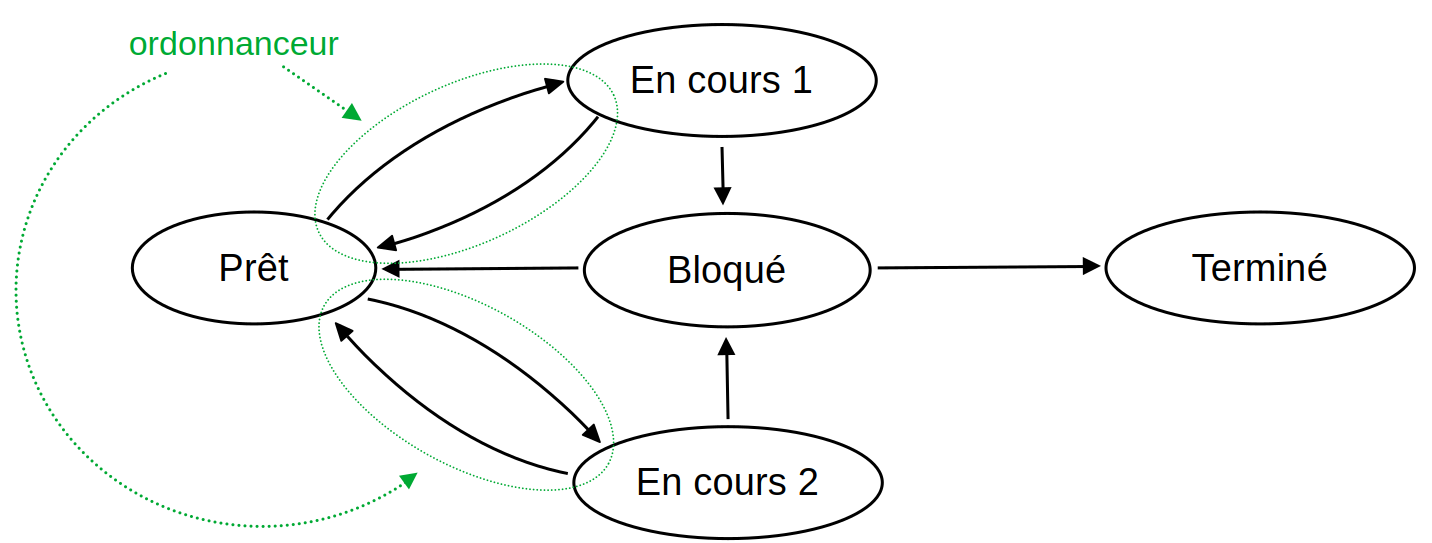
\includegraphics[width=0.9\linewidth]{lecon/17-ordonnancement/graphe_etat.png}\\
	Cycle de vie d'un processus
\end{center}

\begin{com}
	A faire. Mais à comparer avec le truc de Malory, parfois mieux que notre truc à nous.
\end{com}